\section{Data formats for System Biology models}
	\begin{itemize}
		\item formats
		\subitem SBML
		\subitem CellML
		\subitem \sedml
		\item everything in XML
		\item semantic annotations
	\end{itemize}
	\todo{look at STATS paper/MOST for version statistics}

\section{Detecting differences in VCS}
	\subsection{Unix Diff}
	\begin{itemize}
		\item Based on solving the longest common subsequence problem
		\item "The program diff reports differences between two files, expressed as a minimal list of line changes to bring either file into agreement with the other" \cite{Hunt1976}
		\item "The central algorithm of diff solves the ‘longest common subsequence problem’ to find the lines that do not change between files" \cite{Hunt1976}
	\end{itemize}
	
	\subsection{XML Diff}
	cf. Cobena2002 \cite{Cobena2002} and \cite{Waltemath2013} in section 2.2.1
	Chawathe et al., 1996 \cite{Chawathe1996}
	\begin{itemize}
		\item "With flat information deltas may be represented simply as sets of tuples or records inserted into, deleted from, and updated in relations. In hierarchical information, we want to identify changes not just to the 'nodes' in the data, but also to their relationships." \cite{Chawathe1996}
		\item "General-purpose version control systems attempt to handle any kind of document and thus make no assumptions about the underlying document format. Usually, those systems distinguish between binary documents and text documents. Appropriate diff algorithms are employed to detect changes between two versions of a document. Those diff algorithms are either line based (for text documents) or byte based (for binary documents). General-purpose version control systems provide good control for line-organized text documents such as source code or latex documents. For XML documents, where the organization into lines can be neglected, 2 line-based version control is inappropriate." \cite{Ronnau2005}
		\item requirements
			\subitem "Within a delta, the exact location of the change must be identified." \cite{Ronnau2005}
			\subitem "XML Structure Information. An XML document is generally a hierarchically structured document, and can be represented in a tree structure. However, an XML document has other features that distinguish it from a general labeled tree. X-Diff introduces the	notion of node signature and a new matching between the trees corresponding to the two versions of a 	document. Together, these two features are used to find the minimum-cost matching and generate a minimum-cost edit script that is capable of transforming the original version of the document to the new version." \cite{Wang2003}
			\subitem "Unordered Trees. Since XML documents can be represented as trees, the change detection problem is related to the problem of change detection on trees." \cite{Wang2003}
		\item "It [the algorithm] tries to detect (large) subtrees that were left unchanged between the old and new versions. These are matched. Starting from there, the algorithm tries to match more nodes by considering ancestors and descendants of matched nodes and taking labels into consideration. Our algorithm also takes advantage of the specificities of XML data. For instance, it knows of attributes and attribute updates and treat them differently from element or text nodes. It also takes into account ID attributes to match elements." \cite{Cobena2002}
	\end{itemize}
	
	\subsection{BiVeS}
	\begin{itemize}
		\item benefits of XyDiff compared to unix-diff
		\subitem problems with XML
		\subitem no deeper "understanding"
		\item cf. \cite{Waltemath2013} (Oxford 2012), \cite{Scharm2015}
		\item algorithm (list of quotes from \cite{Scharm2015})
		\subitem two versions of an XML-encoded model are translated into an internal tree structure. For every node n in the tree, a hash sum n r and a weight n x are calculated 
		\subitem The weight of a node is thus always greater than the weight of its children. As such, the weight represents the size of the corresponding subtree 
		\subitem The hash sum of a node n represents the signature of the subtree rooted at n 
		\subitem While n r unambiguously defines the subtree rooted in n, n r does not need to be unique among all nodes in the tree. Thus, if n r ¼ m r then the subtrees in n and m are identically equal 
		\subitem First, nodes are being mapped with respect to their identifiers 
		\subitem id attributes in the XML documents serve as identifiers. In addition, we also evaluate biological identifiers, specifically links into bio-ontologies 
		\subitem Second, the initial mapping is propagated upwards into the trees. 
		\subitem The connections of a node’s children are evaluated in a depth-first traversal of T 2 . If a node n in T 2 is connected to a node m in T 1 then a mapping of parent ðnÞ to parent ðmÞ is suggested 
		\subitem If, in contrast, n is not connected, we examine the candidates that were previously suggested by the connections of n’s children. 
		\subitem Candidates which have a different tag name than n and candidates which al- ready have a connection are neglected. 
		\subitem Among the remaining candidates, the algorithm chooses the one that received the best suggestions and connects it to n 
		\subitem Third, the algorithm makes use of the initially computed signatures and maps nodes of T 2 on nodes of T 1 
		\subitem A priority queue U is maintained to sort the nodes of T 2 based on their weights. Initially, U only consists of the root node of T 2 . 
		\subitem Unless U is empty, the algorithm repeatedly removes node n 2 U  T 2 with the biggest weight, which represents the biggest subtree in the queue 
		\subitem Fourth, the algorithm improves the quality of the mapping by examining the network structure of T 1 and T 2 in a top-down approach. For every mapping n 2 T 2 on m 2 T 1 , it compares unmatched children of n and m to find missed mappings 
		\subitem The algorithm evaluates the matrix greedily and adds new mappings up to a maximum distance of 0.9. Thus, nodes which have nothing in common will not be connected 
		\subitem Additional mapping rules capture the domain characteristics of the processed data. Following the current specifications for SBML and CellML, we prohibit certain changes in the hierarchical tree of document nodes. Specifically, we treat parts of the model as atomic con- structs for which we define restrictions on possible network operations 
		\subitem This step is a major reason why our algorithm outperforms standard XML diff algorithms. 
		\subitem insert if an entity is present in T 2 but absent in T 
		\subitem delete if an entity is present in T 1 but absent in T 
		\subitem move if a node is present in both documents, but either (i) the parents in the corresponding trees are not connected or (ii) the parents are connected, but the sequence of their siblings has changed 
		\subitem update if the value of an attribute, a text node's content or the tag name of a node was modified
		\subitem After the mapping, we distinguish two types of nodes: mapped nodes and unmapped nodes. Unmapped nodes n 2 T 1 [ T 2 are nodes for which the algorithm could not find a matching node in the opposite tree. These nodes and their attributes correspond to either inserts or deletes, depending on their origin 
		\subitem In contrast, mapped nodes are nodes for which the algorithm did find a matching node in the opposite tree. If the parents of such a mapping of n 2 T 2 onto m 2 T 1 are not connected, or if the se- quence among their siblings has changed, then these nodes are included in the set of moves 
	\end{itemize}
	
\section{Managing Versions}
	\subsection{Traditional Version Control Systems}
	\begin{itemize}
		\item benefits of version control systems
			\subitem \todo{elaborate}
			\subitem "The need for model version control has been previously discussed in research groups facing model evolution in computational biology (Beard et al., 2009; Cuellar et al., 2006; Hucka et al., 2010; Li et al., 2010; Miller et al., 2011). In general, VCSs such as Subversion (http://subversion.apache.org/) (SVN)" \cite{Waltemath2013}
		\item simple file storage
			\subitem storing files next to each other in the file system
			\subitem "-version1", "-version2", "-final"
			\subitem no meta information stored along with versions (author, time stamp)
			\subitem collaboration causes problems
			\subitem but: simple and quick
		\item SVN
			\subitem client/server architecture
			\subitem collaboration possible, through branching and merging capability
			\subitem reverse-delta storage
			\subitem no offline work possible
		\item GIT
			\subitem distributed VCS
			\subitem reverse-delta storage with version graph
			\subitem build for heavy collaboration by using information from the version graph for merging
			\subitem \todo{refer to version-graph later, when explaining db concept}
			\subitem \url{https://git-scm.com/book/en/v2/Git-Internals-Plumbing-and-Porcelain}
	\end{itemize}
		
	\subsection{Challenges traditional VCS face with Systems Biology models}
	\begin{itemize}
		\item SVN and GIT are using unix-diff -> not suitable for XML files (cf. XML diff section)
		\item no semantic information about the changes (cf. comodi)
		\item no domain specific knowledge to improve mapping of different XML-tree branches
			\subitem important for good detection of tree branch movement etc. 
			\subitem "A model VCS should be tailored to existing model representation formats, which are typically XML and RDF based. It should furthermore reflect the temporal evolution of a model and present model changes to the users." \cite{Waltemath2013}
			\subitem "These
			common changes are detected by the LCS algorithm, but they are in fact irrelevant for the model’s history and would be neglected by entity-based algorithms. In other words, although being successfully used for source code version control, LCS is not suitable for XML version control (Chawathe et al., 1996)." \cite{Waltemath2013}
		\item As proposed in \cite{Waltemath2013} there are 2 major approaches to keep track of changes:
			\subitem keeping track of (minor) changes in the model itself
			\subitem tracking versions in the repository
	\end{itemize}


\section{Ontologies in Computer Science}

	\begin{itemize}
	\item definition
		\subitem formal definition, properties and relation of entities
	\item use of BioOntologies cf. Courtot
	\end{itemize}

	\todo{cite owl standard, when explaining comodi import}
	\todo{http://msb.embopress.org/content/7/1/543.short for ontology overview}
	
	\subsection{COMODI}
	\begin{itemize}
		\item cf. \cite{Scharm2016}
	\end{itemize}
	
\section{Using graph databases to store \sysbio models}
	\label{sec:graph-db}
	\begin{itemize}
		\item \masymos exists
		\item graph databases (eg. neo4j) are more suitable for inhomogeneous data
		\item queries are easier
	\end{itemize}
	
	\subsection{Graph Databases}
	\begin{itemize}
		\item \todo{explain neo4j}
	\end{itemize}
	
	\subsection{Graph Database schema and the Entity Relation model}
	\label{sec:graph-db:er}
	Relational databases have established a supremacy over the time, it is therefore well known, how to convert formal modeling approaches like entity-relationship (ER) models and UML class diagrams into a relational schema. With introducing so called noSQL databases, which break with classic relational design, modeling schema got. Mostly because they do not favor a defined data structure.
	But since 
	Even though neo4j, introduced in section \ref{sec:graph-db}, is part of the schema-free noSQL 
	\begin{itemize}
	\item entities:
		\subitem name of the entity becomes vertex name (neo4j node label)
		\subitem associated attributes become vertex properties
	\item relations:
		\subitem binary relations:
			\subsubitem become edge type
			\subsubitem name of relation becomes the edge label
			\subsubitem associated attributes become edge properties
			\subsubitem end-point of the edge-type are the vertex-type corresponding to the related entity type
		\subitem n-ary relations:
			\subsubitem name of the relation becomes name of a \emph{new} vertex type
			\subsubitem associated attributes become the properties of the vertex type
			\subsubitem new vertex-type includes edges to vertex-types corresponding to the related entity-types
			\subsubitem these edges are labeled after the role of the participating entity in the relationship
			\subsubitem directions do not matter
	\item cf. \cite{Siriwaradhana2014}
	\end{itemize}
	
	\begin{figure}
		\center
		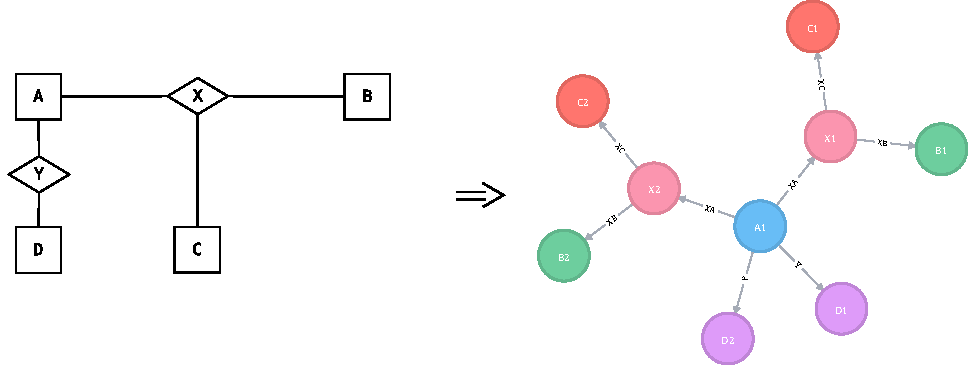
\includegraphics[height=150pt]{resources/er-to-neo4j.pdf}
		\caption{Example conversion of an ER diagram into a neo4j graph}
	
		%Create (a1:A {name: 'A1'}), (b1:B {name: 'B1'}), (b2:B {name: 'B2'}), (c1:C {name: 'C1'}), (c2:C {name: 'C2'}), (d1:D {name: 'D1'}), (d2:D {name: 'D2'}), (x1:X {name: 'X1'}), (x2:X {name: 'X2'}), (a1)-[:XA]->(x1), (x1)-[:XB]->(b1), (x1)-[:XC]->(c1), (a1)-[:Y]->(d1), (a1)-[:Y]->(d2), (a1)-[:XA]->(x2), (x2)-[:XB]->(b2), (x2)-[:XC]->(c2)
		
		\label{fig:example-er-diagram}
	\end{figure}
	
	\subsection{\masymos}
	% following some quotes from the Henkel2015 paper
	\begin{itemize}
	\item This work is based on MaSyMoS, "a graph database for simulation models and associated data" \cite{Henkel2015}
		\subitem \cite{Henkel2015} Many models in public databases encode networks that can be represented as graphs
		\subitem \cite{Henkel2015} relational databases were developed for homogeneous, structured data, e.g. numerical data
		\subitem \cite{Henkel2015} Designing a relational representation for these links and keeping the database effi\item cient at the same time are impossible
	
	\item \cite{Henkel2015} MaSyMos is a database based on neo4j for storing and retrieving structural information of biological models
		\subitem \cite{Henkel2015} We chose the graph database Neo4J (25)
		\subitem \cite{Henkel2015} follows the fundamental properties of databases, i.e. the ACID principles
		
	\item \cite{Henkel2015} biological models are represented in heterogenous data structures e.g. networks. Traditional relational databases are build to quickly process highly structured data in tables, therefore they are less efficient in storing and retrieving standard encoded models, due to their highly linked structure
		\subitem \cite{Henkel2015} No unified schema exists for models and meta-data, making it difficult to define a relational database schema
		\subitem \cite{Henkel2015} highly linked models, model entities and meta-data are difficult to represent in a table-based relational database
	\item \masymos data model and structure
		\subitem \cite{Henkel2015} document root node is created for each data item
		\subitem each model is represented by a model node
			\subsubitem entry point for each model import is a document node
		\subitem \cite{Henkel2015} Attached to the model node are annotation nodes, including the reference publication
		\subitem in SBML compartments, species and reactions are linked to the model node
		\subitem in CellML each component is linked to the model node, further containing variables and mathematical relationships to manipulate other variables
			\subsubitem \cite{Henkel2015} component contains vari- ables and mathematical relationships that manipulate those variables
		\subitem Experiment setups are stored under a SEDML node, instead of a model node. In comparison to species, reactions, compartments or components the SEDML node has links to Modelreference nodes, as well as nodes pointing to different model entities used in plots. Nevertheless no processing information is stored in the database.
			\subsubitem \cite{Henkel2015} SEDML node serves as the anchor for an experiment
			\subsubitem \cite{Henkel2015} Modelreference node links the experiment to all Model nodes used in the simulation
			\subsubitem \cite{Henkel2015} do not store the specific processing of a model entity
		\subitem Semantic annotations and cross-references from the models are stored as seperate nodes and linked to the ontology node representing the used ontology term.
			\subsubitem \cite{Henkel2015} Semantic annotations and cross-references
			\subsubitem \cite{Henkel2015} We parse these ontologies and add all concepts and relations as nodes and edges, respectively.
		\subitem ensure an easy traversal upwards, a connection is created from each node of the stored model that points to the parent of the current node. The corresponding edges are named belongsTo]
	\item Linking model related data
		\subitem main advantage to prior mentioned storage in relational databases is the possibility to flexibly link data between different domains. //Henkel et al.// describes 3 different links, which are currently implemented: 1. links between (model) annotations and the corresponding ontology term 2. links between models or model entities and SEDML simulation descriptions or respectively SEDML variables 3. links between model entities in different standard format representation
			\subsubitem \cite{Henkel2015} The main advantage of the previously described concept is its possibility to define flexible links between the data do\item mains)
			\subsubitem \cite{Henkel2015} links between annotations (in SBML, CellML and SED-ML) and ontology concepts)
			\subsubitem \cite{Henkel2015} links between models (in SBML or CellML format) and SED-ML
			\subsubitem \cite{Henkel2015} link is that between a model and a simulation description
			\subsubitem \cite{Henkel2015} links between model entities and SED-ML variables
			\subsubitem \cite{Henkel2015} links between model entities from different model rep- resentation formats
		\subitem \cite{Henkel2015} For each annotation in a model we add an explicit link to the data entry in the ref- erenced bio-ontology
		\subitem This link is shared between all models using this annotation, regardless of the format
		\subitem Further to explicit links (one hop in the graph), MaSyMoS is able to determine implicit links between different models. Those can be established over shared resources like a publication, publication author or annotations with common bio-ontologies. Regarding a publications the database may establish connections based on the likelihood of names by Hemming Distance, resulting in a confidence which can be increased, "" if the entities' annotations match
			\subsubitem \cite{Henkel2015} In addition, we determine implicit links between models of different representation formats
			\subsubitem \cite{Henkel2015} If two models share a publication, the systems can infer implicit links between those entities that are equally named
	\item Implementation
		\subitem MaSyMoS is designed to run as both standalone commandline application with embedded neo4j and as an extension to the neo4j server. Latter is controlled by an unmanaged neo4j plugin providing a RESTful json interface.
		\subitem Same interface also cooperates with the retrieval engine Morre, by providing endpoints to query different search indexes.
		
	\item MaSyMoS project structure
		\subitem The MaSyMoS project is divided into 3 different modules: MaSyMoS-core, Morre and a CLI.
		\subitem The core module contains the logic of the database and communicates directly with neo4j. It consists of routines and a Java API to import models, experiments and ontologies. Further it fetches linked information from common bio-ontologies and manages, updates and queries Lucene indexes.
		\subitem The Command Line Interface (CLI) provides a user interface, to easily interact with the API provided by the core module. It's main purpose was to simplify the development process by skipping the deployment step. Instead it is possible to directly interact with and debug MaSyMoS
		\subitem The Morre module is similiar to the CLI, by providing an way to interact with the core. But instead of providing a user interface, Morre is loaded as neo4j unmanaged extension and exposes a RESTful interface, which can be used to query the Lucene indexes or to push and update models to the database.
	\end{itemize}
	\todo{Pictures}
	
